\section{Progettazione}

\subsection{Layout}

Si è cercato di utilizzare un layout che si avvicina alla maggior parte dei 
siti web cosi che l'utente ha un senso di familiarità a prima vista.

Si può suddividere ogni pagina in quattro aree principali, 
partendo dall'alto verso il basso si può vedere

\begin{itemize}
	\item \textit{Header}:  visualizzerà i link alle pagine
	corrispondenti alle principali funzionalità del sito, compresi il login e la registrazione;
	\item \textit{Breadcrumb}: situato appena sotto l'header, tiene traccia del 
	percorso che fa l'utente visualizzandola e si può ritornare nelle posizioni precedenti;
	\item \textit{Main}: è il contenuto principale della pagina, cambiera' in base alla pagina visualizzata;
	\item \textit{Footer}: la parte finale dove verrà visualizzata gli autori del sito web
\end{itemize}


\subsection{Accessibilità}

Per quanto riguarda l'accessibilità, si è prestato particolarmente attenzione a:

\begin{itemize}
	\item \textit{Immagini}: le immagini presenti nel sito hanno un testo alternativo che le descrive
	cosi da aiutare gli utenti con disablità visive.

	Pultroppo non si assicura che tutti testi alternativi
	siano ben curati e che diano una descrizione utile, in quanto ci sono casi in cui sono 
	gli utenti stessi a caricare le immagini, anche se viene richiesto di inserire una descrizione;
	un esempio è quando un utente fa una richiesta di assistenza nella pagina di Riparazione;
	\item \textit{Lingua}: la lingua principale del sito e' Italiano quindi le parole straniere che 
	si presenti saranno marcate con la loro lingua di appartenenza;
	\item \textit{Colori}: i colori dei testi e sottofondo hanno un buon contrasto tra di loro.
	Inoltre come richiesto dagli standard, i colori dei link visitati sono diversi da quelli non visitati.
	
	Di seguito vengono elencati i colori utilizzati e il contrasto tra di loro:

	\begin{tabular}{| C{4.5cm} | C{4.5cm} | C{4.5cm} |}
		\hline
		\textbf{Testo} & \textbf{Sottofondo} & \textbf{Contrasto}\\
		\hline
		\#152238 & \#D0D0DC & 10.42\\
		\#551A8B & \#D0D0DC & 7.2\\
		\#152238 & \#FFFFFF & 15.93\\
		\#FFFFFF & \#2a792d & 5.42\\
		\#FFFFFF & \#af2b1d & 6.59\\
		\hline
	\end{tabular}\\
	
	\item \textit{Font}: il font utilizzato è chiaro e semplice;

	\begin{figure}[H]
	\centering
	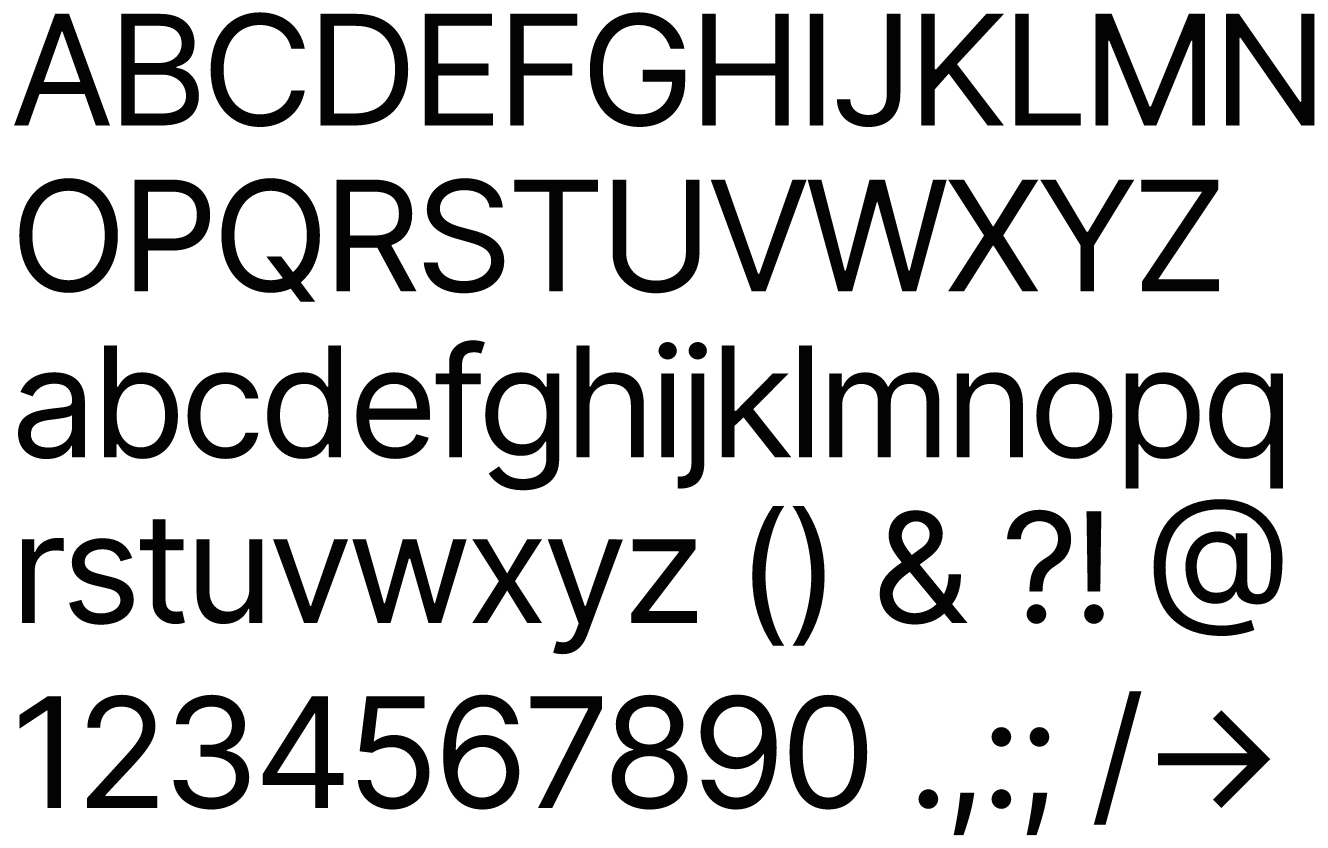
\includegraphics[scale=0.4]{res/font.png}
	\caption{Font Utilizzato}
	\end{figure}

	\item \textit{Struttura}: la struttura del sito è poco profonda, è possibile raggiungere ogni pagina
	del sito web con massimo tre click;
	\item \textit{Posizione}: nel breadcrumb e' stato aggiungo all'inizio il testo \textit{"Ti trovi in:"} per l'orientamento;
	\item \textit{Flessibilita'}: il sito risponde ai ridimensionamenti, cambiando il design in base al dispositivo utilizzato;
\end{itemize}

	

